\chapter{Related Work}
\label{ch:related_work}
This chapter describes the current state of the stepper motor controllers in the Robotics group and the efforts to improve it.
Ongoing efforts to use program embedded systems in the Rust programming language is also described, both in the context of our research group and also in general.
Finally, similar projects - either software or hardware wise are reported.

\section{KM2}
\label{sec:km2}
In the Robotics and AI research group, currently a second generation of the KM2 stepper motor controller is widely in use.
A render of the KM2 controller can be seen in the figure~\ref{fig:km2render}.
It is used primarily by the students of the BPC-PRP course for driving a simple differentially driven robot.
The controller utilizes an ATMega8 paired with two stepper motor controllers DRV8825, that are utilized in the form of breakout boards generally used in the now obsolete RAMPS boards.
The motor controller is controlled using the I\textsuperscript{2}C bus.
There are two major shortcomings of the driver - the used controller's I\textsuperscript{2}C peripheral's clock-stretching is not compatible with Raspberry Pi's, causing problems on clock speeds higher than 30 kHz.
The second shortcoming are the used driver chips, that are quite loud and do not support contemporary advanced features.
The boards for 3D printers are also reportedly not well designed and they may \hl{overheat}~\cite{prusa_rambo}.

\begin{figure}[H]
    \centering
    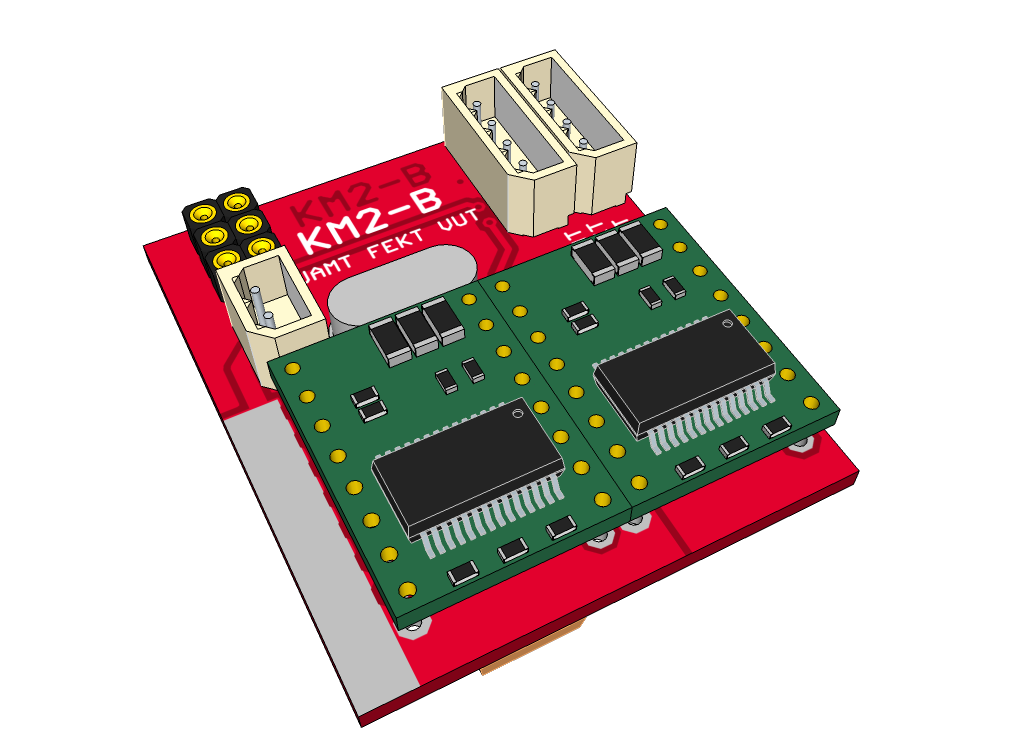
\includegraphics[width=0.5\textwidth]{obrazky/km2render}
    \caption{KM2 motor controller render~\cite{km2render}.}
    \label{fig:km2render}
\end{figure}

\section{KM3}
\label{sec:km3}
The KM3 (or KM2-C) was supposed to be a successor to the previously described KM2 controllers and it aimed to mainly solve the clock stretching problem by utilizing an STM32F031 MCU.
Another advantage of this revision was that the breakout boards for motor driver chips were replaced with driver chips soldered directly on the driver PCB (Printed Circuit Board).
The controller can be seen in the figure~\ref{fig:km3}.
Even though the new MCU was an improvement over the ATMega8, it proved to be the bottleneck for implementing new functionality to the motor controller as the MCU has very limited memory, both FLASH and RAM and peripherals.
For example, the lack of pins made it impossible to directly generate pulses to control the STEP/DIR interface of the motor drivers chip and the control had therefore be done manually in software.
Also the fact, that the MCU utilizes a Cortex-M0 core means that the support for atomic instructions mis missing, making it hard to work with guarantees about memory safety in cases of interrupt routine being called during memory manipulation

We developed the firmware~\cite{km3-firmware} for this board and concluded that the board and its design may be suitable for the students' robot projects, but it is way too limited to be used in more serious projects.
We also concluded that the hardware used is now overcome and the development of this board shall not be further pursued.

\begin{figure}[H]
    \centering
    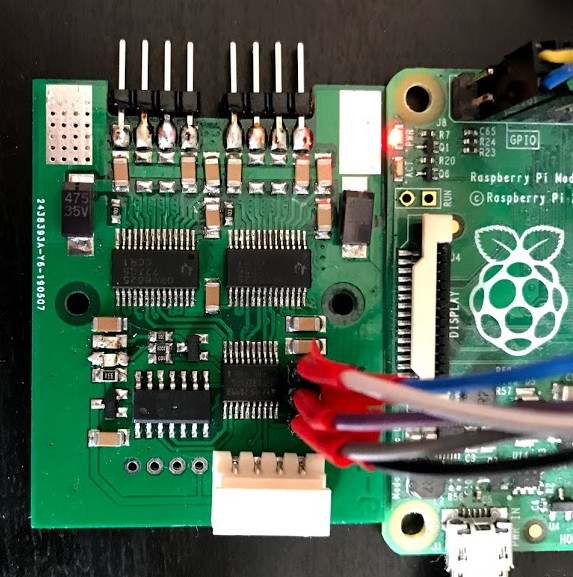
\includegraphics[width=0.7\textwidth]{obrazky/km3}
    \caption{The KM3 motor controller connected to a Raspberry Pi~\cite{km2render}.}
    \label{fig:km3}
\end{figure}

\section{DC motor}
\label{sec:dcmotor}

\section{Mechaduino}
\label{sec:mechaduino}

\section{Flott}
\label{sec:flott}
